\documentclass[letterpaper,12pt]{scrartcl}
\usepackage{epsfig,latexsym,amsmath,amssymb,epic,eepic,psfrag,subfigure,float,euscript,array}
\usepackage[latin1]{inputenc}
\usepackage[margin=24mm]{geometry}
\usepackage{enumitem}
\usepackage{tikz,pgf,pgfplots}
\usepgfplotslibrary{fillbetween}
\usepgfplotslibrary{groupplots}
\usetikzlibrary{decorations, arrows}

\usepackage[amssymb]{SIunits}

\newenvironment{exercise}[1][Problem]{\begin{trivlist} \item[\hskip
    \labelsep {\stepcounter{exerctr}\bfseries #1
      \arabic{exerctr}}]}{\end{trivlist}\vspace{10mm}}

\newcounter{exerctr}
\newcounter{abcctr}[exerctr]

\newcommand{\abc}{\noindent\vspace{1mm}\\ {\bf
    \stepcounter{abcctr}(\alph{abcctr})\ }}
\newcommand{\bbm}{\begin{bmatrix}}
\newcommand{\ebm}{\end{bmatrix}}
\newcommand{\point}[1]{\hfill {\bf (#1p)}\\ \vspace{-5mm}}
\newcommand{\ctrb}{\EuScript{S}}
\newcommand{\Lap}{\mathcal{L}}
\newcommand{\obsv}{\EuScript{O}}
\newcommand{\realdel}{\text{Re}}
\newcommand{\imagdel}{\text{Im}}
\newcommand{\bC}{\mathbb{C}}
\newcommand{\bR}{\mathbb{R}}
\newcommand{\bmpv}{\begin{minipage}[t]}
\newcommand{\bmps}{\begin{minipage}[t]{45mm}}
\newcommand{\bmpm}{\begin{minipage}[t]{90mm}}
\newcommand{\bmpl}{\begin{minipage}[t]{\textwidth}}
\newcommand{\emp}{\end{minipage}}
\newcommand{\mexp}[1]{\ensuremath{\mathrm{e}^{#1}}}
\newcommand*{\laplaceinv}[1]{\ensuremath{\mathcal{L}^{-1} \left\{#1\right\}}}
\newcommand*{\ztrf}[1]{\ensuremath{\mathcal{Z} \left\{#1\right\}}}

\newcommand{\AxisRotator}[1][rotate=0]{%
    \tikz [x=0.2cm,y=0.60cm,line width=.1ex,-stealth,#1] \draw (0,0) arc (-150:150:1 and 1);%
}

\newcommand{\shift}{\ensuremath{\operatorname{q}}}
%\addtolength{\topmargin}{-1cm}
%\textheight 22.5cm
%\oddsidemargin 1.3cm
%\evensidemargin 1.3cm

\makeatletter
\newcommand*{\rom}[1]{\expandafter\@slowromancap\romannumeral #1@}
\makeatother

\newcommand*\circled[1]{\tikz[baseline=(char.base)]{
            \node[shape=circle,draw,inner sep=2pt] (char) {#1};}}


\pgfplotstableread[col sep=comma]{dc-motor-pid-timeseries.dat}\outputtable

\title{Computerized Control partial exam 1 (18\%)}
\author{Kjartan Halvorsen}
\date{}

\begin{document}

\maketitle


\begin{description}
\item[Time] September 19 19:05-20.35
\item[Place] 5305
\item[Permitted aids] The single colored page with your own notes, table of Laplace transforms, calculator
\end{description}

All answers should be readable and well motivated (if nothing else is written). Solutions/motivations should be written on the provided spaces in this exam. Use the last page if more space is needed.

\begin{center}
{\Large Good luck!} \\
\end{center}

\noindent
\fbox{
\bmpl
{\bf Matricula and name:}\\
\vspace*{14mm}
\emp}


%\clearpage

%-----------------------------------------------------------------

\subsection*{Position servo for a DC-motor}
Consider a DC-motor connected to a load. The differential equation describing the dynamics of the system is
\begin{equation}
  T \ddot{y}(t) + \dot{y}(t)  = bu(t) + v(t),
\label{eq:ode}
\end{equation}
where $y(t)$ is the angle of the shaft, $u(t)$ is the voltage applied to the circuit and $v(t)$ is a torque disturbance on the shaft. The time-constant of the system is $T$ and $b$ is a gain parameter. We want to control the angle of the shaft using a simple proportional controller.
\begin{center}
  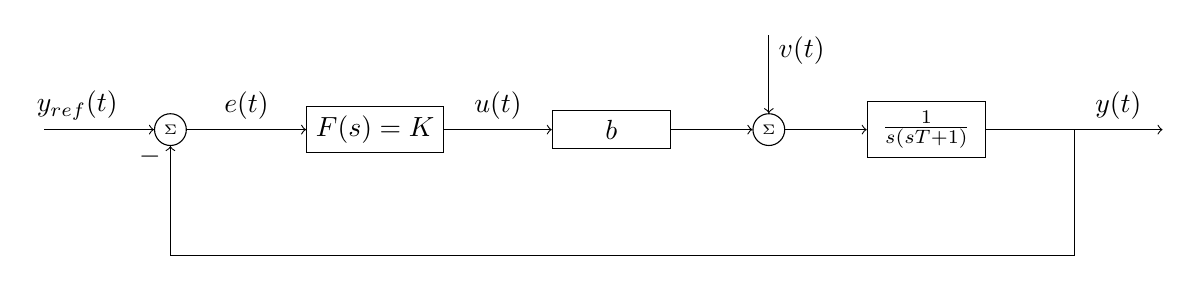
\begin{tikzpicture}[node distance=22mm, block/.style={rectangle, draw, minimum width=15mm}, sumnode/.style={circle, draw, inner sep=2pt}]
      
      \node[coordinate] (input) {};
      \node[sumnode, right of=input, node distance=16mm] (sum) {\tiny $\Sigma$};
      \node[block, right of=sum, node distance=26mm] (controller)  {$F(s)=K$};
      \node[block, right of=controller, node distance=30mm] (plantgain)  {$b$};
      \node[sumnode, right of=plantgain, node distance=20mm] (sumdist)  {\tiny $\Sigma$};
      \node[block, right of=sumdist, node distance=20mm] (plant)  {$\frac{1}{s(sT+1)}$};
      \node[coordinate, above of=sumdist, node distance=12mm] (disturbance) {};
      \node[coordinate, right of=plant, node distance=30mm] (output) {};

      \draw[->] (input) -- node[above, pos=0.3] {$y_{ref}(t)$} (sum);
      \draw[->] (sum) -- node[above] {$e(t)$} (controller);
      \draw[->] (controller) -- node[above] {$u(t)$} (plantgain);
      \draw[->] (plantgain) -- node[above] {} (sumdist);
      \draw[->] (sumdist) -- node[above] {} (plant);
      \draw[->] (plant) -- node[coordinate] (measure) {} node[above, near end] {$y(t)$} (output);
      \draw[->] (disturbance) -- node[right, pos=0.2] {$v(t)$} (sumdist);
      \draw[->] (measure) -- ++(0,-16mm) -|  node[pos=0.95, left] {$-$} (sum);
    \end{tikzpicture}
  \end{center}
  

\begin{exercise}
  \abc%
  Sketch a root locus showing how the poles of the continous-time, closed-loop system depend on the controller gain $K$.

\noindent
  \begin{tikzpicture}
    \begin{axis}[
      axis lines = middle,
      xmin=-10, xmax=3,
      ymin=-2, ymax=2,
      xtick=\empty,
      ytick=\empty,
      xlabel=Re,
      ylabel=Im,
      ]
    \end{axis}
  \end{tikzpicture}
%
%  \abc%
%  For what values of the gain $K$ is the closed-loop system stable?
%
%\noindent
%\fbox{
%\bmpl
%{\bf Answer:}\\
%\vspace*{35mm}
%\emp}
 
 \abc%
  Mark in the root locus above the location of a set of  closed-loop poles (one on each branch) that gives the best performance possible with proportional control. Motivate your choice!

\noindent\fbox{
\bmpl
{\bf Motivation:}\\
\vspace*{35mm}
\emp}
 
\end{exercise}


\begin{exercise} % Sampling of the plant
 The controller we are actually going to use is implemented on a microcontroller. So to be able design a controller taking into account the discrete-time nature of the closed-loop system, we want to work with a discrete-time model of the plant.  
\abc
Show that zero-order-hold sampling of the DC-motor gives the pulse-transfer function
\[ H(z) = \frac{B(z)}{A(z)} = \frac{T\big(\frac{h}{T}-1+\mexp{-\frac{h}{T}}\big)z + T\big(1-\mexp{-\frac{h}{T}}-\frac{h}{T}\mexp{-\frac{h}{T}}\big)}{(z-1)\big(z-\mexp{-\frac{h}{T}}\big)}.\]
You may have use of the identity \(\frac{1}{s^2(sT+1)} = \frac{T^2}{sT+1} - \frac{T}{s} + \frac{1}{s^2}\).

\noindent
\fbox{
\bmpl
{\bf Calculations:}\\
\vspace*{161mm}
\emp}

\abc State as a mathematical expression how the continuous-time poles (in the s-plane) and the corresponding discrete-time poles (in the z-plane) are related, and verify that the relationship holds in this particular case.

\noindent
\fbox{
\bmpl
{\bf Answer:}\\
\vspace*{30mm}
\emp}

%\abc A common rule-of-thumb used to choose a sampling period is that we should have 4 to 10 samples per rise time of the plant or the closed-loop system: \(t_rh \approx\) 4 --- 10. Suggest a suitable sampling period for the DC-motor described by \eqref{eq:ode}.
%
%\noindent
%\fbox{
%\bmpl
%{\bf Answer:}\\
%\vspace*{30mm}
%\emp}


\end{exercise}

\begin{exercise} % Discrete-time P-control
Consider now doing proportional  control in discrete time.
\begin{center}
  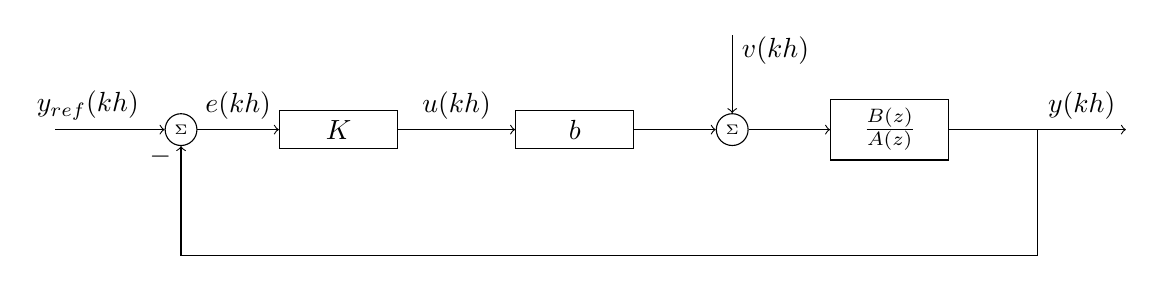
\begin{tikzpicture}[node distance=22mm, block/.style={rectangle, draw, minimum width=15mm}, sumnode/.style={circle, draw, inner sep=2pt}]
      
      \node[coordinate] (input) {};
      \node[sumnode, right of=input, node distance=16mm] (sum) {\tiny $\Sigma$};
      \node[block, right of=sum, node distance=20mm] (controller)  {$K$};
      \node[block, right of=controller, node distance=30mm] (plantgain)  {$b$};
      \node[sumnode, right of=plantgain, node distance=20mm] (sumdist)  {\tiny $\Sigma$};
      \node[block, right of=sumdist, node distance=20mm] (plant)  {$\frac{B(z)}{A(z)}$};
      \node[coordinate, above of=sumdist, node distance=12mm] (disturbance) {};
      \node[coordinate, right of=plant, node distance=30mm] (output) {};

      \draw[->] (input) -- node[above, pos=0.3] {$y_{ref}(kh)$} (sum);
      \draw[->] (sum) -- node[above] {$e(kh)$} (controller);
      \draw[->] (controller) -- node[above] {$u(kh)$} (plantgain);
      \draw[->] (plantgain) -- node[above] {} (sumdist);
      \draw[->] (sumdist) -- node[above] {} (plant);
      \draw[->] (plant) -- node[coordinate] (measure) {} node[above, near end] {$y(kh)$} (output);
      \draw[->] (disturbance) -- node[right, pos=0.2] {$v(kh)$} (sumdist);
      \draw[->] (measure) -- ++(0,-16mm) -|  node[pos=0.95, left] {$-$} (sum);
    \end{tikzpicture}
  \end{center}
We simplify the pulse-transfer function of the DC-motor by writing
\[ H(z) = \frac{B(z)}{A(z)} = \frac{T(\mexp{-\frac{h}{T}}-1 + \frac{h}{T})z + T(1-\mexp{-\frac{h}{T}} - \frac{h}{T}\mexp{-\frac{h}{T}})}{(z-1)(z-\mexp{-\frac{h}{T}})} = \frac{b_0z + b_1}{(z-1)(z-p)}. \]
Using the approximation $\mexp{-\frac{h}{T}} \approx 1 - \frac{h}{T} + 0.5(\frac{h}{T})^2$, the  approximate location of the zero is
\begin{align*}
 z &= - \frac{b_1}{b_0} = \frac{\mexp{-\frac{h}{T}} -1 + \frac{h}{T}\mexp{-\frac{h}{T}}}{\mexp{-\frac{h}{T}}-1 + \frac{h}{T}}
   \approx \frac{1 - \frac{h}{T} + 0.5(\frac{h}{T})^2 -1  + \frac{h}{T}(1 - \frac{h}{T} + 0.5(\frac{h}{T})^2)}{1 - \frac{h}{T}  + 0.5(\frac{h}{T})^2 -1 + \frac{h}{T}}\\
   &= \frac{-0.5(\frac{h}{T})^2 + 0.5(\frac{h}{T})^3}{0.5(\frac{h}{T})^2} = -1 + 0.5\frac{h}{T},
\end{align*}
which  for reasonable sampling periods $h$ is inside the unit circle and close to -1.
%\[ z = - \frac{b_1}{b_0} = \frac{\mexp{-\frac{h}{T}} -1 + \frac{h}{T}\mexp{-\frac{h}{T}}}{\mexp{-\frac{h}{T}}-1 + \frac{h}{T}} = \frac{\mexp{-\frac{h}{T}} -1 + \frac{h}{T} - \frac{h}{T} + \frac{h}{T}\mexp{-\frac{h}{T}}}{\mexp{-\frac{h}{T}}-1 + \frac{h}{T}} =  1 - \frac{\frac{h}{T}(1-\mexp{-\frac{h}{T}})}{\mexp{-\frac{h}{T}}-1 + \frac{h}{T}},\]
\abc%
Show that the closed-loop pulse-transfer function from the disturbance $v(kh)$ to the output $y(kh)$ is
\[H_{cv}(z) = \frac{b_0z + b_1}{(z-1)(z-p) + Kb(b_0z + b_1)}.\]

\noindent
\fbox{
\bmpl
{\bf Calculations:}\\
\vspace*{85mm}
\emp}
\abc%
  Sketch a root locus showing how the poles of the discrete-time closed-loop system depend on the controller gain $K$.

\noindent
  \begin{tikzpicture}
    \def\axlim{1.8}
    \begin{axis}[
      width=8cm, height=8cm,
      axis equal,
      axis lines = middle,
      xmin=-\axlim, xmax=\axlim,
      ymin=-\axlim, ymax=\axlim,
      xtick=\empty,
      ytick=\empty,
      xlabel=Re,
      ylabel=Im,
      ]
      \addplot[no marks, samples=300, domain=0:360] ({cos(x)}, {sin(x)});
    \end{axis}
  \end{tikzpicture}
  \abc%
  Will the closed-loop system be stable for any value  of the gain $K$?

\noindent
\fbox{
\bmpl
{\bf Answer and motivation:}\\
\vspace*{15mm}
\emp}

  \abc%
  Mark in  your root locus for the discrete-time system the location of a set of  closed-loop poles (one on each branch) that gives the best performance possible with proportional control. Motivate your choice!

\noindent\fbox{
\bmpl
{\bf Motivation:}\\
\vspace*{35mm}
\emp}

%\abc
%[Bonus problem worth 5p] Use the final-value theorem 
%\[ \lim_{k\to\infty} y(kh) = \lim_{z\to 1} (1-z^{-1})Y(z)\]
%to determine the steady-state error in the angle $y(kh)$ for a unit step disturbance $v(kh)$. Can you suggest  (no calculations needed) another controller that will improve the steady-state error? 
 
%\noindent\fbox{
%\bmpl
%{\bf Calculation  and answer:}\\
%\vspace*{55mm}
%\emp}

\end{exercise}
\begin{exercise} % Different values of K, pair pole map to step response.
For a particular DC-motor with time-constant $T=1$, gain $b=1$, and using the sampling period $h=\unit{0.2}{\second}$, the following discrete-time PID-controller is proposed
\[ F(z) = K\frac{6 z^2 - 11 z + 5.2}{z^2 -1.2z + 0.2}. \]
\abc%
With the suggested PID-controller and $K=1$ we get the loop-gain $L(z) = H(z)F(z)$, whose frequency response is shown in the Bode diagram and Nyquist plot below. Determine (numerical values) and indicate (mark in the plots) the following: Crossover frequency ($\omega_c$), phase margin ($\varphi_m$), phase-crossover frequency ($\omega_p$) and amplitude margin ($A_m$)
\begin{center}
  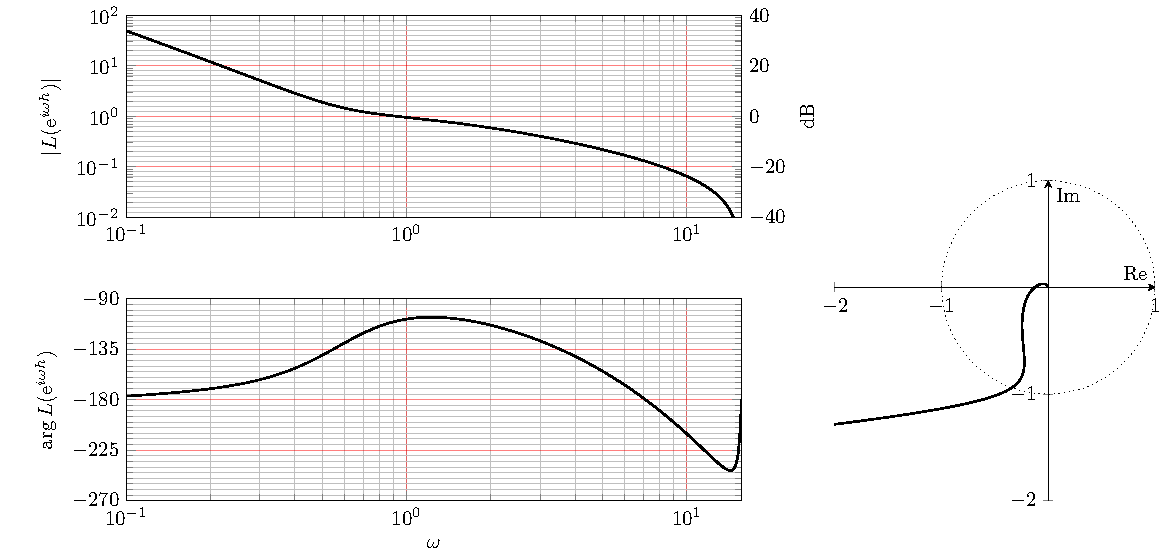
\includegraphics[width=\linewidth]{bode-nyquist-dc-pid}
\end{center}

\noindent\fbox{
\bmpl
\begin{tabular}{l@{=}p{5cm}l@{=}p{4cm}}
$\omega_c$ & & $\varphi_m$&\\[5mm]
$\omega_p$ & & $A_m$&\\[2mm]
\end{tabular}
\emp}

\abc%
The root locus of the closed-loop system w.r.t~the gain $K$ is given below
\begin{center}
\begin{tikzpicture}
    \node[anchor=south west,inner sep=0] at (0,0) {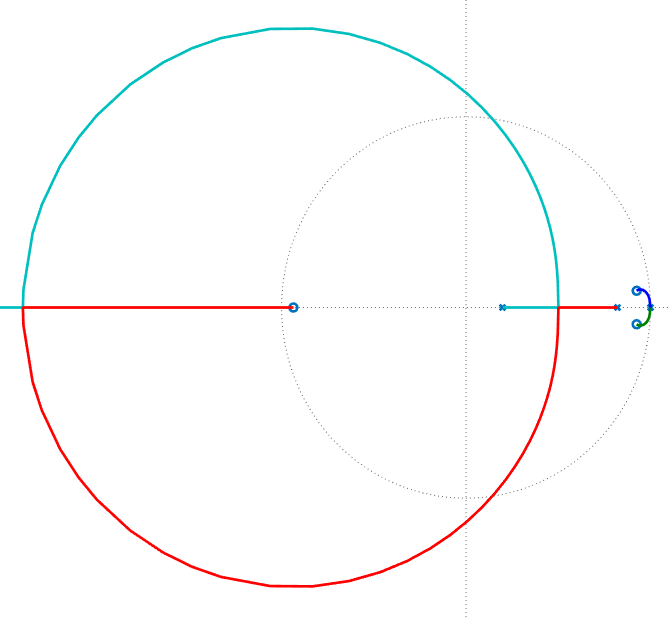
\includegraphics[width=0.5\linewidth]{rlocus-pid-dc-motor.png}};
    \node[coordinate, pin={[pin distance=20mm] 10:{$K=7.8$}}] at (6.16,6.28) {};
\end{tikzpicture} 
\end{center}
In figure~\ref{fig:responses}, four different closed-loop responses to a step in the reference angle $y_{ref}$ are shown. The different responses are for four different values of $K$. Identify (and circle) the corresponding step plot for each value of $K$ in the table below. \textbf{Motivate your choice!}
\begin{center}
\begin{tabular}{cl}
\(K\) & Step plot\\\hline
0.5 & I\hspace*{2mm} II\hspace*{2mm} III\hspace*{2mm} IV\\[1mm]
1.0 & I\hspace*{2mm} II\hspace*{2mm} III\hspace*{2mm} IV\\[1mm]
2.0 & I\hspace*{2mm} II\hspace*{2mm} III\hspace*{2mm} IV\\[1mm]
6.0 & I\hspace*{2mm} II\hspace*{2mm} III\hspace*{2mm} IV\\ \hline
\end{tabular}
\end{center}


%\tikzset{plttype/.style={ycomb, thick, mark=*, mark options={red!60!black}}}
\tikzset{plttype/.style={const plot, no marks, ultra thick}}

\begin{figure}[h]
\begin{center}
\begin{tikzpicture}[node distance=2cm]

\begin{groupplot} [
    group style={
      group name=timeplot,
      group size=2 by 2,
      xlabels at=all,
      horizontal sep=2cm,
      vertical sep=2cm,
    }, 
    clip=false,
    height=4.3cm, width=8.3cm,
    axis line style={->},
    axis lines=left,
    xlabel={$k$ },
    ylabel={$y(k)$},
      %grid=both,
      % xtick=\empty,
      % ytick=\XNOLL,
      % yticklabel=$x_0$,
      ]
      \nextgroupplot
      \addplot[plttype] table[y = 3] from \outputtable ;
 \nextgroupplot
\addplot[plttype] table[y = 1] from \outputtable;
 \nextgroupplot
\addplot[plttype] table[y = 2] from \outputtable ;
 \nextgroupplot
\addplot[plttype] table[y = 4] from \outputtable ;
\end{groupplot}

\node[red!80!black!90] at ($ (timeplot c1r1.north) + (5mm, -5mm) $) {\huge \rom{1}};
\node[red!80!black!90] at ($ (timeplot c1r2.north) + (5mm, -5mm) $) {\huge \rom{2}};
\node[red!80!black!90] at ($ (timeplot c2r1.north) + (5mm, -5mm) $) {\huge \rom{3}};
\node[red!80!black!90] at ($ (timeplot c2r2.north) + (5mm, -5mm) $) {\huge \rom{4}};

  \end{tikzpicture}
  \caption{Step-responses of the closed-loop system.}
  \label{fig:responses}
\end{center}

\end{figure}

\noindent
\fbox{
\bmpl
{\bf Motivation:}\\
\vspace*{60mm}
\emp}

\abc
[Bonus problem worth 5p] If the gain is $K=7.8$ the closed-loop system will have two complex-conjugated poles on the unit circle (see the root locus), and the response of the system will have undamped oscillations. What will be the \emph{period} of  these oscillations (in seconds)? \emph{Hint:} For $K=7.8$, the Nyquist curve passes through the point -1.
 
\noindent\fbox{
\bmpl
{\bf Calculation and answer:}\\
\vspace*{55mm}
\emp}

\end{exercise}


\cleardoublepage
%\end{document}

\section*{Solutions}
\setcounter{exerctr}{0} 

\begin{exercise}
\abc We have loop gain
\[ L(s) = KG(s) = K \frac{\overbrace{1}^{Q(s)}}{\underbrace{s(sT+1)}_{P(s)}}, \]
and the characteristic equation 
\[ s(sT+1) + K = 0\] for the closed-loop system. We have $n=2$ start points ($s=0$, $s=-\frac{1}{T}$) and $m=0$ end points. The $n-m=2$ asymptotes have directions $\pm \frac{\pi}{2}$, and intersects the real axis in the point \[i.p. = \frac{\sum p_i - \sum q_i}{n-m} = \frac{ 0 - \frac{1}{T_i}}{2} = - \frac{1}{2T_i}. \] The root locus looks like below
\begin{center}
\begin{tikzpicture}
  \draw[->] (-4,0) -- node[below, very near end] {Re} (2,0);
  \draw[->] (0,-4) -- node[right, very near end] {Im} (0,4);
  \draw[red!80!black, thick] (-2,0) -- (-1,0) -- (-1,4);
  \draw[red!80!black, thick] (0,0) -- (-1,0) -- (-1,-4);
  \node[red!80!black]  at (-2,0) {$\times$};
  \node[red!80!black]  at (0,0) {$\times$};
  \draw (-2,0) -- (-2, -0.2) node[below] {$-\frac{1}{T}$};
%  \draw (0,1) -- (0.2, 1) node[below] {$\frac{i}{2T}$};
\end{tikzpicture}
\end{center}
\abc Good performance in general means fast and well-damped response. Assuming that some small overshoot in the step-response  is acceptable, we may aim for the fastest possible poles with a damping ratio of $\zeta=0.707$. This means poles which have imaginary part equal in magnitude to the real part. Note that for the pure continuous-case the system will stay stable (but be more and more oscillatory) no matter how large we choose the gain $K$.
\begin{center}
\begin{tikzpicture}
  \draw[->] (-4,0) -- node[below, very near end] {Re} (2,0);
  \draw[->] (0,-4) -- node[right, very near end] {Im} (0,4);
  \draw[red!80!black, thick] (-2,0) -- (-1,0) -- (-1,4);
  \draw[red!80!black, thick] (0,0) -- (-1,0) -- (-1,-4);
  \node[red!80!black]  at (-2,0) {$\times$};
  \node[red!80!black]  at (0,0) {$\times$};
  \draw (-2,0) -- (-2, -0.2) node[below] {$-\frac{1}{T}$};
  \draw (0,1) -- (0.2, 1) node[right] {$\frac{i}{2T}$};
  \draw (0,-1) -- (0.2, -1) node[right] {$-\frac{i}{2T}$};
  \node[]  at (-1,1) {\Large $\times$};
  \node[]  at (-1,-1) {\Large $\times$};
\end{tikzpicture}
\end{center}
\end{exercise}

\begin{exercise}
\abc First we calculate the step-response of the DC-motor
\begin{align*}
  y(t) &= \laplaceinv{\frac{1}{s(sT + 1)} \frac{1}{s}} = \laplaceinv{\frac{1}{s^2(sT+1)}}\\
  &= \laplaceinv{\frac{T^2}{sT+1} - \frac{T}{s} + \frac{1}{s^2}} = \laplaceinv{\frac{T^2}{sT+1}} - \laplaceinv{\frac{T}{s}} + \laplaceinv{\frac{1}{s^2}}\\
&= T\mexp{-\frac{t}{T}} - T + t, \quad t \ge 0.
\end{align*}
Then we sample (set $t=kh$), and find the z-transform
\begin{align*}
  Y(z) &= \ztrf{T\mexp{-\frac{h}{T}k}} - T\ztrf{u_H(k)} + \ztrf{kh}\\
       &=  \frac{zT}{z-\mexp{-\frac{h}{T}}} - \frac{zT}{z-1}  + \frac{zh}{(z-1)^2}.
\end{align*}
Finally, form the pulse-transfer function
\begin{align*}
  H(z) &= \frac{Y(z)}{U(z)} = \frac{z-1}{z} \left( \frac{zT}{z-\mexp{-\frac{h}{T}}} - \frac{zT}{z-1}  + \frac{zh}{(z-1)^2}\right)\\
      &= \frac{T(z-1)}{z-\mexp{-\frac{h}{T}}} - T + \frac{h}{(z-1)}\\
      &= \frac{T(z-1)^2 -T(z-1)(z-\mexp{-\frac{h}{T}}) + h(z-\mexp{-\frac{h}{T}})}{(z-1)(z-\mexp{-\frac{h}{T}})}\\
      &= \frac{T(z^2 - 2z + 1) - T(z^2 - (1+\mexp{-\frac{h}{T}})z + \mexp{-\frac{h}{T}}) + hz - h\mexp{-\frac{h}{T}}}{(z-1)(z-\mexp{-\frac{h}{T}})}\\
      &= \frac{T(\mexp{-\frac{h}{T}}-1 + \frac{h}{T})z + T(1-\mexp{-\frac{h}{T}} - \frac{h}{T}\mexp{-\frac{h}{T}})}{(z-1)(z-\mexp{-\frac{h}{T}})},
\end{align*}
which correponds to the one given.
\abc When we sample a plant using ZOH, the poles are related through the expression \(z = \mexp{sh}\). The continuous-time poles of the DC-motor are $s_1=0$ and $s_2 = -\frac{1}{T}$, so using the expression we get
\[ z_1 = \mexp{s_1h} = \mexp{0} = 1, \qquad z_1 = \mexp{s_2h} = \mexp{-\frac{h}{T}},\]
which are exactly the poles of the discrete-time pulse-transfer function.
\end{exercise}

\begin{exercise}
  \abc Using Mason's rule we have that the closed-loop pulse-transfer function is
  \[ H_{cv}(z) = \frac{\frac{B(z)}{A(z)}}{1 + Kb\frac{B(z)}{A(z)}} = \frac{B(z)}{A(z) + KbB(z)} = \frac{b_1z + b_1}{(z-1)(z-p) + Kb(b_0z + b_1)}.\]

  \abc There are $n=2$ start points in $z=1$ and $z=p=\mexp{-\frac{h}{T}}$, and one end-point in the open-loop zero $z = -1 + 0.5\frac{h}{T}$. There is one asymptote with direction $\pi$. The part of the real axis between the two startpoints belongs to the root locus (the ``odd rule'') and also everything to the left of the end point. This means that the two branches must meet between the two start points, then branch out into the imaginary plane, loop to the left and meet again on the negative real axis outside the unit circle. After this, one branch goes toward infinity and one goes to the end point. It should look something like below
\begin{center}
  \begin{tikzpicture}
    \def\axlim{1.8}
    \begin{axis}[
      width=8cm, height=8cm,
      axis equal,
      axis lines = middle,
      xmin=-\axlim, xmax=\axlim,
      ymin=-\axlim, ymax=\axlim,
      xtick=\empty,
      ytick=\empty,
      xlabel=Re,
      ylabel=Im,
      clip=false,
      ]
      \addplot[no marks, samples=300, domain=0:360] ({cos(x)}, {sin(x)});
      \addplot[green!60!black, thick,no marks,] coordinates { (0.7,0) (0.85,0)};
      \addplot[red!60!black, thick,no marks,] coordinates { (1,0) (0.85,0)};
      \addplot[blue!80!black, thick,no marks, samples=300, domain=0:180] ({(-1.8+0.85)+1.8*cos(x))}, {1.8*sin(x)});
      \addplot[orange!80!black, thick,no marks, samples=300, domain=0:-180] ({(-1.8+0.85)+1.8*cos(x))}, {1.8*sin(x)});
      \addplot[yellow!60!black, thick,no marks,] coordinates { (0.85-3.6,0) (-0.9,0)};
      \addplot[magenta!60!black, thick,no marks,] coordinates { (0.85-3.6,0) (-5,0)};
      
      \node[red!60!black] at (axis cs: 1,0) {\large $\times$};
      \node[green!60!black] at (axis cs: 0.7,0) {\large $\times$};
      \node[cyan!40!black] at (axis cs: -0.9,0) {\large $\circ$};


    \end{axis}
  \end{tikzpicture}
\end{center}

\abc No, clearly there is a limited range of gains $K$ for which the system is stable. This is in contrast to the continuous-time case, where the system is stable for any gain $K$.

\abc With similar motivation as for the continous-time case, we want as fast system as possible with not too much oscillations. So complex-conjugated poles as far from $z=1$ as possible, but with some distance to the unit circle is reasonable.
\begin{center}
  \begin{tikzpicture}
    \def\axlim{1.8}
    \begin{axis}[
      width=8cm, height=8cm,
      axis equal,
      axis lines = middle,
      xmin=-\axlim, xmax=\axlim,
      ymin=-\axlim, ymax=\axlim,
      xtick=\empty,
      ytick=\empty,
      xlabel=Re,
      ylabel=Im,
      clip=false,
      ]
      \addplot[no marks, samples=300, domain=0:360] ({cos(x)}, {sin(x)});
      \addplot[green!60!black, thick,no marks,] coordinates { (0.7,0) (0.85,0)};
      \addplot[red!60!black, thick,no marks,] coordinates { (1,0) (0.85,0)};
      \addplot[blue!80!black, thick,no marks, samples=300, domain=0:180] ({(-1.8+0.85)+1.8*cos(x))}, {1.8*sin(x)});
      \addplot[orange!80!black, thick,no marks, samples=300, domain=0:-180] ({(-1.8+0.85)+1.8*cos(x))}, {1.8*sin(x)});
      \addplot[yellow!60!black, thick,no marks,] coordinates { (0.85-3.6,0) (-0.9,0)};
      \addplot[magenta!60!black, thick,no marks,] coordinates { (0.85-3.6,0) (-5,0)};
      
      \node[red!60!black] at (axis cs: 1,0) {\large $\times$};
      \node[green!60!black] at (axis cs: 0.7,0) {\large $\times$};
      \node[cyan!40!black] at (axis cs: -0.9,0) {\large $\circ$};


      \node[black] at (axis cs: 0.83,0.3) {\Large $\times$};
      \node[black] at (axis cs: 0.83,-0.3) {\Large $\times$};

    \end{axis}
  \end{tikzpicture}
\end{center}

\end{exercise}

\begin{exercise}
\abc%
\begin{center}
  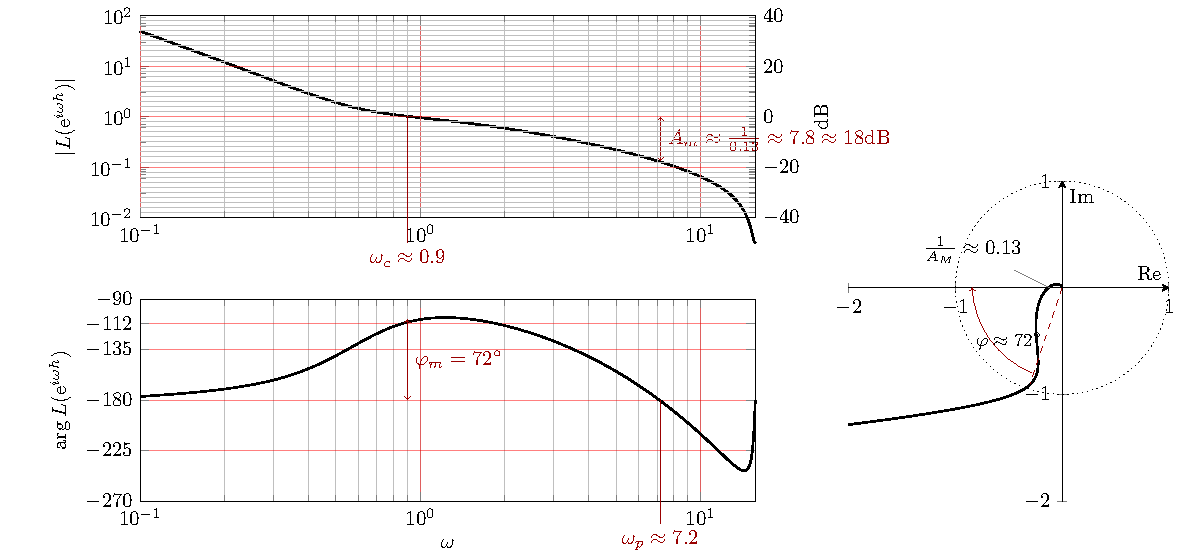
\includegraphics[width=\linewidth]{bode-nyquist-dc-pid-sol}
\end{center}
\abc From the root locus we see that we have four starting points. Two start points are in $z=1$ (one from the pole of the DC-motor and one from the integrator of the PID controller), and two start points are well inside the unit circle. For small gains $K$, the behaviour will be dominated by the two slow poles close to $z=1$. These two poles will never become unstable, but approach the two end points. The two poles starting inside the unit circle will meet and the for the gain  $K=7.8$ they will break out of the unit circle and the closed-loop system will be unstable. This means that for small gains the closed-loop system will be slow, and somewhat oscillatory (slow oscillations), with increasing gains, the response will be better damped initially, until the two poles (on the red and cyan branches) gets closer to the unit circle, which will give a response with fast and poorly damped oscillations. With this motivation, the answer becomes
\begin{center}
\begin{tabular}{cl}
\(K\) & Step plot\\\hline
0.5 & I\hspace*{2mm} II\hspace*{2mm} \circled{III}\hspace*{2mm} IV\\
1.0 & I\hspace*{2mm} \circled{II}\hspace*{2mm} III\hspace*{2mm} IV\\
2.0 & \circled{I}\hspace*{2mm} II\hspace*{2mm} III\hspace*{2mm} IV\\
6.0 & I\hspace*{2mm} II\hspace*{2mm} III\hspace*{2mm} \circled{IV}\\ \hline
\end{tabular}
\end{center}
In fact, the actual position of the poles for the four different values of the gain $K$ is shown in the root locus below.
\begin{center}
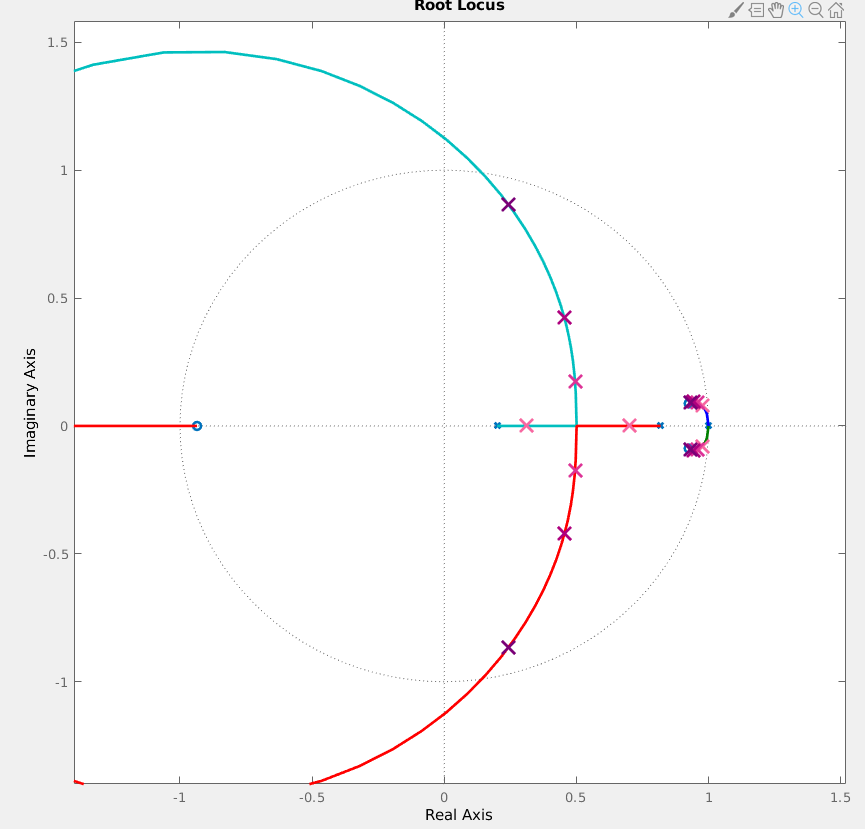
\includegraphics[width=0.8\linewidth]{dc-motor-rlocus-sol.png}
\end{center}

\abc%
Looking at the Bode diagram and Nyquist plot again, we see that the gain $K=7.8$ is the same as the gain margin. So the Nyquist curve goes through the point $-1$ for $\omega = \omega_p \approx \unit{7.2}{\rad\per\second}$, and the closed-loop system will have undamped oscillations with this frequency. In discrete time, this corresponds to a closed-loop system with a pair of complex-conjugated poles on the unit circle at $z=\mexp{\pm i \omega_ph} = \mexp{\pm i 7.2\cdot 0.2} = \mexp{\pm i 1.44}$ which has argument \unit{1.44}{\rad} = \unit{82.5}{\degree}. This is exactly where the rootlocus intersects the unit circle. The period of the oscillations is $T=\frac{2\pi}{7.2} \approx \unit{0.87}{\second}$. 
\end{exercise}
\end{document}
